\documentclass[11pt,a4paper]{article}
\usepackage{notes}
\usepackage{pgfplots}
\usepackage{fancyhdr}

\pagestyle{fancy}
\fancyhf{}
\lhead{Geophysics IIIA: Potential Fields \& Geothermics}
\rhead{Week 5 Isostatic Gravity Correction}
\cfoot{\thepage}

\title{Week 5 --- Activity: Isostatic Gravity Correction}
\author{Geophysics 3A: Potential Fields \& Geothermics}
\date{\today}

\begin{document}
\maketitle

\section*{Purpose}

In this problem, you will derive the isostatic gravity correction under the assumption of Airy isostasy, starting from a Bouguer slab formulation and progressing to a practical implementation using topography and a reference crustal thickness.

\subsection*{Background}

Consider a reference Earth model with a constant crustal thickness $T_0$. Surface topography $h(x)$ is compensated by a crustal root $r(x)$ such that columns of equal width have equal mass above a compensation depth.

Let:
\begin{itemize}
    \item $\rho_c$ = crustal density
    \item $\rho_m$ = mantle density
    \item $h(x)$ = surface elevation
    \item $r(x)$ = additional root thickness relative to $T_0$
\end{itemize}

\subsection*{Geometry}

\begin{figure}[h!]
    \centering
    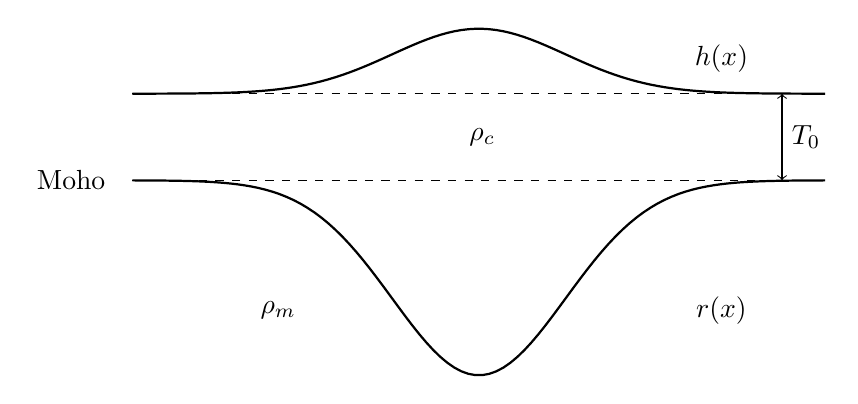
\begin{tikzpicture}[scale=1.1]

    % Parameters
    \def\A{0.75}      % topography amplitude
    \def\Tzero{1.0}  % reference crustal thickness
    \def\k{0.5}      % Gaussian width

    % Topography (Gaussian)
    \draw[thick, domain=-4:4, samples=100]
        plot (\x, {\A*exp(-\k*\x*\x)});

    % Reference surface (sea level)
    \draw[dashed] (-4,0) -- (4,0);

    % Moho (reference crustal thickness)
    \draw[dashed] (-4,-\Tzero) -- (4,-\Tzero);

    % Root (3x amplitude below Moho)
    \draw[thick, domain=-4:4, samples=100]
        plot (\x, {-\Tzero - 3*\A*exp(-\k*\x*\x)});

    % Label topography
    \node at (2.8,0.4) {$h(x)$};

    % Label root
    \node at (2.8,-2.5) {$r(x)$};

    % Label T0 with bracket
    \draw[<->] (3.5,0) -- (3.5,-\Tzero);

    \node[left] at (0.3,-0.5) {$\rho_c$};
    \node[left] at (-2,-2.5) {$\rho_m$};

    \node[right] at (3.5,-0.5*\Tzero) {$T_0$};

    % Label Moho
    \node[left] at (-4.2,-\Tzero) {Moho};

    \end{tikzpicture}
    \caption{A mountain with a topographic expression $h(x)$ and compensating root $r(x)$.}
\end{figure}

\subsection*{Part A: Airy Isostasy}

\begin{enumerate}
    \item Starting from mass balance between a reference column and a column with topography, show that:
    \[
    \rho_c h = (\rho_m - \rho_c) r
    \]

    \item Solve for the root thickness $r(x)$ in terms of $h(x)$.
\end{enumerate}

\subsection*{Part B: Gravity of an Infinite Slab}

The gravitational attraction of an infinite horizontal slab of thickness $t$ and density $\rho$ is:
\[
g = 2\pi G \rho t
\]

\begin{enumerate}
    \setcounter{enumi}{2}
    \item Write an expression for the gravitational effect of the topography.

    \item Write an expression for the gravitational effect of the crustal root. Carefully define the density contrast.
\end{enumerate}

\subsection*{Part C: Substitution and Simplification}

\begin{enumerate}
    \setcounter{enumi}{4}
    \item Substitute your expression for $r(x)$ into the root gravity term.

    \item Show that the total gravity effect of the topography plus its Airy root simplifies to:
    \[
    g_{\text{total}} = 0
    \]
\end{enumerate}

\subsection*{Part D: Practical Isostatic Correction}

In practice, crustal thickness is not known everywhere. Instead, we assume a reference thickness $T_0$ and compute $r(x)$ from observed topography.

\begin{enumerate}
    \setcounter{enumi}{6}
    \item Explain why the isostatic correction is model-dependent.

    \item Write the final expression for the isostatic correction in terms of $h(x)$ only.
\end{enumerate}

\subsection*{Target Result}

You should show that the gravity effect of the compensating root is:
\[
g_{\text{root}} = -2\pi G \rho_c h
\]

and that, under perfect Airy compensation, the combined effect of topography and root cancels exactly.

\subsection*{Extension (Optional)}

Discuss how this result would change if:
\begin{itemize}
    \item compensation were incomplete
    \item the lithosphere behaved elastically (flexural isostasy)
\end{itemize}

\end{document}